\documentclass[12pt, letterpaper]{article}
\usepackage[utf8]{inputenc}
\usepackage{tikz}
\usepackage{pgfplots}

\title{Traveling Sales Person}
\author{Brandon George \thanks{Dr. Nurk for the great starter code and moving the due date!}}
\date{November 2018}

\begin{document}

\begin{titlepage}
\maketitle
\end{titlepage}

\begin{abstract}
Welcome to the Traveling Sales Person Problem! This was my fist attempt at making a GPU program and I think that it has been very beneficial to understanding what GPU programming might look like.
\end{abstract}

\section{Report}

\subsection{Three Cities}
\begin{center}
  \begin{tabular}{|c | c c c c ||}
    \hline
    Cities & $p$ & $t_p$(s) & $s$ & $e$ \\
    \hline\hline
      3 & 1 & 0.063 & - & - \\
       & 2 & 0.050 & 1.26 & .63 \\
       & 4 & 0.050 & 1.26 & .315 \\
       & 6 & 0.050 & 1.26 & .21 \\
      \hline\hline
      \hline
  \end{tabular}
\end{center}
\begin{tikzpicture}
  \begin{axis}[title={$t_p$ versus $p$},xlabel={$p$},ylabel={$t_p$},xmin=1, xmax=6,legend pos=north west, ymajorgrids=true,grid style=dashed]
  \addplot[color=blue,mark=square]coordinates{(1,.063)(2,.05)(4,.05)(6,.05)};
  \end{axis}
\end{tikzpicture}

\subsection{Four Cities}
\begin{center}
  \begin{tabular}{|c | c c c c ||}
    \hline
    Cities & $p$ & $t_p$(s) & $s$ & $e$ \\
    \hline\hline
      4 & 1 & 0.061 & - & - \\
       & 2 & 0.050 & 1.22 & .62 \\
       & 4 & 0.050 & 1.22 & .305 \\
       & 8 & 0.049 & 1.24 & .155 \\
       & 16 & 0.050 & 1.22 & .076 \\
       & 24 & 0.052 & 1.17 & .049 \\
      \hline\hline
      \hline
  \end{tabular}
\end{center}
\begin{tikzpicture}
  \begin{axis}[title={$t_p$ versus $p$},xlabel={$p$},ylabel={$t_p$},xmin=1, xmax=24,legend pos=north west, ymajorgrids=true,grid style=dashed]
  \addplot[color=blue,mark=square]coordinates{(1,.061)(2,.05)(4,.05)(8,.049)(16,.05)(24,.052)};
  \end{axis}
\end{tikzpicture}

\subsection{Five Cities}
\begin{center}
  \begin{tabular}{|c | c c c c ||}
    \hline
    Cities & $p$ & $t_p$(s) & $s$ & $e$ \\
    \hline\hline
      5 & 1 & 0.050 & - & - \\
       & 2 & 0.051 & .98 & .49 \\
       & 4 & 0.050 & 1 & .25 \\
       & 8 & 0.065 & .76 & .095 \\
       & 16 & 0.063 & .76 & .048 \\
       & 32 & 0.050 & 1 & .0313 \\
       & 64 & 0.050 & 1 & .016 \\
       & 120 & 0.050 & 1 & .008 \\
      \hline\hline
      \hline
  \end{tabular}
\end{center}
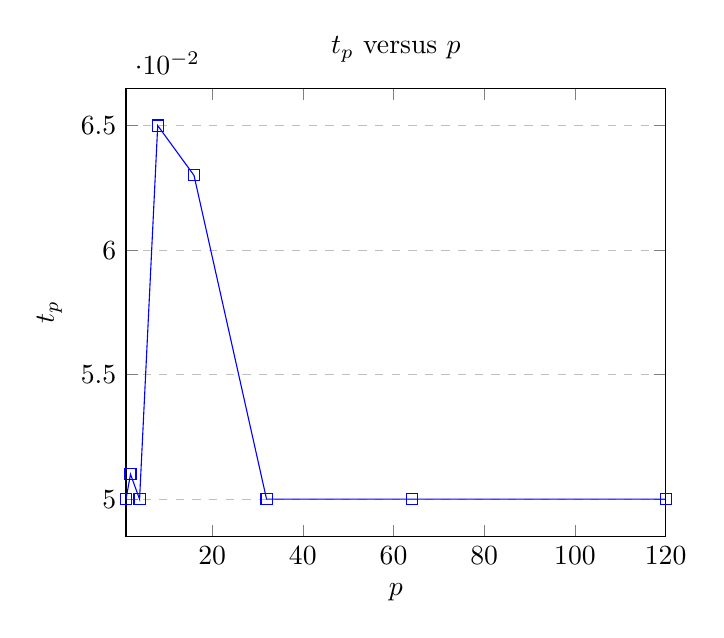
\begin{tikzpicture}
  \begin{axis}[title={$t_p$ versus $p$},xlabel={$p$},ylabel={$t_p$},xmin=1, xmax=120,legend pos=north west, ymajorgrids=true,grid style=dashed]
  \addplot[color=blue,mark=square]coordinates{(1,.05)(2,.051)(4,.05)(8,.065)(16,.063)(32,.05)(64,.05)(120,.05)};
  \end{axis}
\end{tikzpicture}

\subsection{Six Cities}
\begin{center}
  \begin{tabular}{|c | c c c c ||}
    \hline
    Cities & $p$ & $t_p$(s) & $s$ & $e$ \\
    \hline\hline
      6 & 1 &  0.053& - & - \\
       & 2 &  0.051& 1.03 & .515 \\
       & 4 &  0.052& 1.01 & .2525 \\
       & 8 &  0.051& 1.03 & .129 \\
       & 16 & 0.052 & 1.01 & .063 \\
       & 32 & 0.051 & 1.03 & .032 \\
       & 64 & 0.051 & 1.03 & .016 \\
       & 128 &0.051  & 1.03 & .008 \\
       & 256 &0.051  & 1.03 & .004 \\
       & 512 &0.052  & 1.01 & .002 \\
       & 720 &0.053  & 1 & .001 \\
      \hline\hline
      \hline
  \end{tabular}
\end{center}
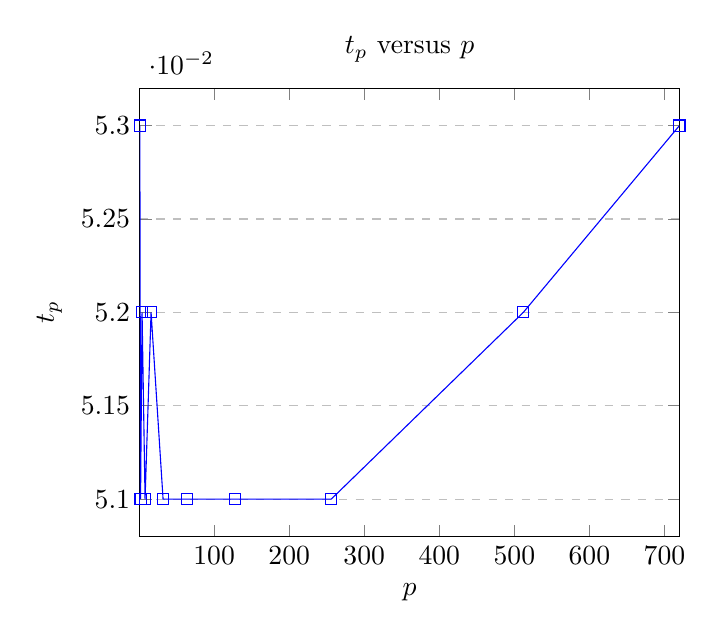
\begin{tikzpicture}
  \begin{axis}[title={$t_p$ versus $p$},xlabel={$p$},ylabel={$t_p$},xmin=1, xmax=720,legend pos=north west, ymajorgrids=true,grid style=dashed]
  \addplot[color=blue,mark=square]coordinates{(1,.053)(2,.051)(4,.052)(8,.051)(16,.052)(32,.051)(64,.051)(128,.051)(256,.051)(512,.052)(720,.053)};
  \end{axis}
\end{tikzpicture}

\subsection{Seven Cities}
\begin{center}
  \begin{tabular}{|c | c c ||}
    \hline
    Cities & $p$ & $t_p$(s) \\
    \hline\hline
      7 & 4 &  0.056\\
       & 8 &  0.053\\
       & 16 & 0.052 \\
       & 32 & 0.052 \\
       & 64 & 0.055 \\
       & 128 &0.055  \\
       & 256 &0.052  \\
       & 512 &0.052  \\
       & 1024 & 0.067 \\
      \hline\hline
      \hline
  \end{tabular}
\end{center}
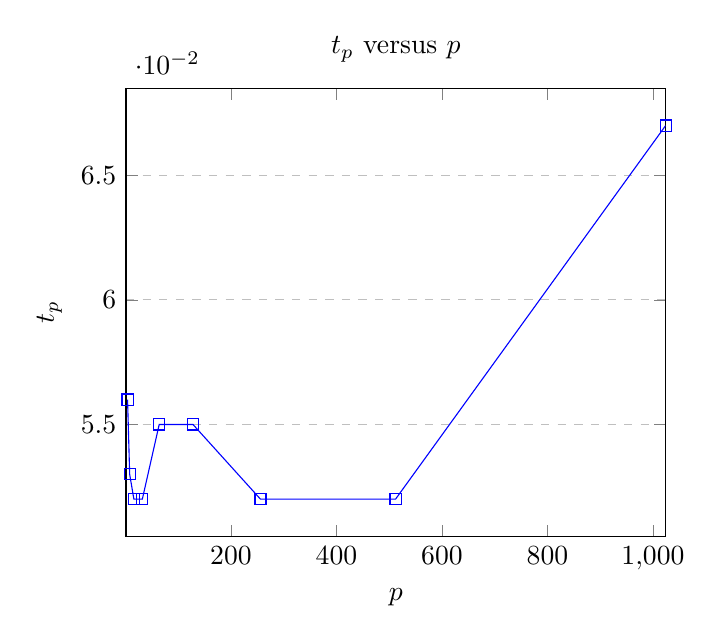
\begin{tikzpicture}
  \begin{axis}[title={$t_p$ versus $p$},xlabel={$p$},ylabel={$t_p$},xmin=1, xmax=1024,legend pos=north west, ymajorgrids=true,grid style=dashed]
  \addplot[color=blue,mark=square]coordinates{(4,.056)(8,.053)(16,.052)(32,.052)(64,.055)(128,.055)(256,.052)(512,.052)(1024,.067)};
  \end{axis}
\end{tikzpicture}

\subsection{Eight Cities}
\begin{center}
  \begin{tabular}{|c | c c ||}
    \hline
    Cities & $p$ & $t_p$(s)\\
    \hline\hline
      8 & 8 &  0.071\\
       & 16 & 0.061 \\
       & 32 & 0.057 \\
       & 64 & 0.053 \\
       & 128 &0.053  \\
       & 256 &0.052  \\
       & 512 &0.052  \\
       & 1024 & 0.053 \\
      \hline\hline
      \hline
  \end{tabular}
\end{center}
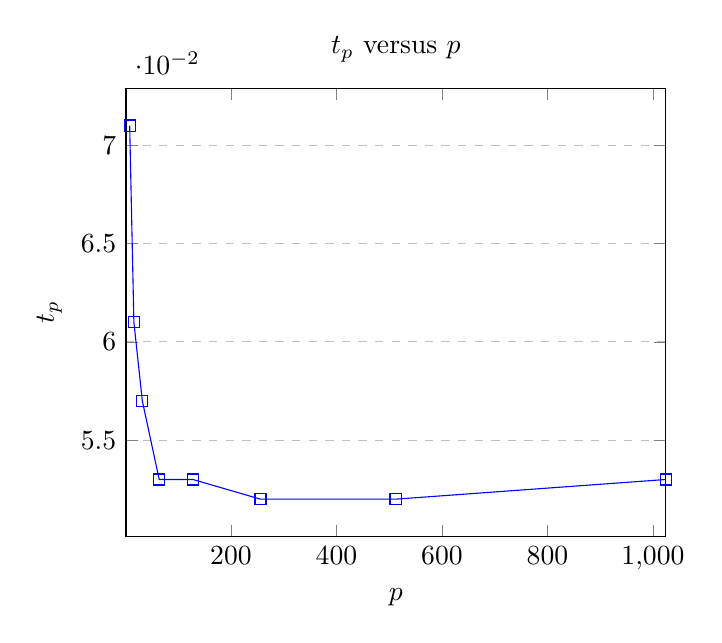
\begin{tikzpicture}
  \begin{axis}[title={$t_p$ versus $p$},xlabel={$p$},ylabel={$t_p$},xmin=1, xmax=1024,legend pos=north west, ymajorgrids=true,grid style=dashed]
  \addplot[color=blue,mark=square]coordinates{(8,.071)(16,.061)(32,.057)(64,.053)(128,.053)(256,.052)(512,.052)(1024,.053)};
  \end{axis}
\end{tikzpicture}

\subsection{Nine Cities}
\begin{center}
  \begin{tabular}{|c | c c ||}
    \hline
    Cities & $p$ & $t_p$(s)\\
    \hline\hline
      9 & 8 &  0.259\\
       & 16 & 0.156 \\
       & 32 & 0.109 \\
       & 64 & 0.081 \\
       & 128 &0.069  \\
       & 256 &0.062  \\
       & 512 &0.059  \\
       & 1024 & 0.063 \\
      \hline\hline
      \hline
  \end{tabular}
\end{center}
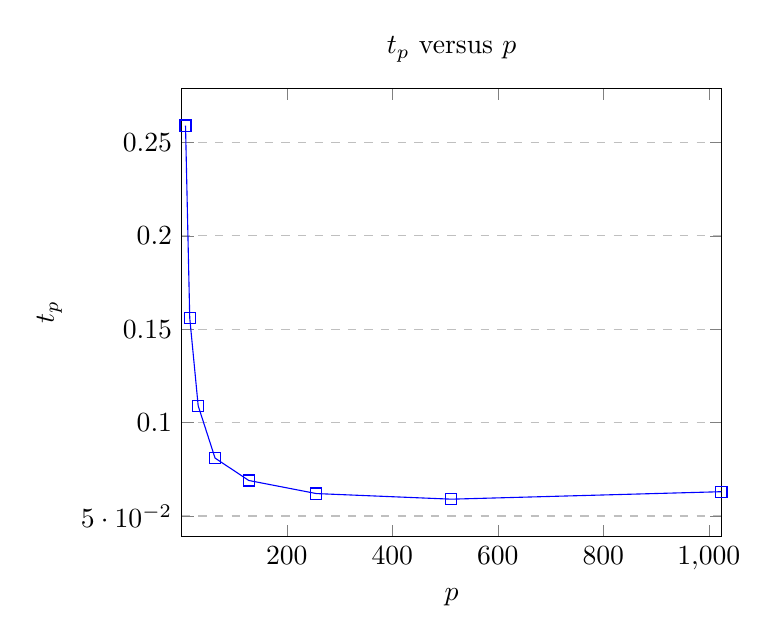
\begin{tikzpicture}
  \begin{axis}[title={$t_p$ versus $p$},xlabel={$p$},ylabel={$t_p$},xmin=1, xmax=1024,legend pos=north west, ymajorgrids=true,grid style=dashed]
  \addplot[color=blue,mark=square]coordinates{(8,.259)(16,.156)(32,.109)(64,.081)(128,.069)(256,.062)(512,.059)(1024,.063)};
  \end{axis}
\end{tikzpicture}

\subsection{Ten Cities}
\begin{center}
  \begin{tabular}{|c | c c ||}
    \hline
    Cities & $p$ & $t_p$(s)\\
    \hline\hline
      10 & 8 &  2.336\\
       & 16 & 1.240 \\
       & 32 & 0.700 \\
       & 64 & 0.386 \\
       & 128 &0.225  \\
       & 256 &0.156  \\
       & 512 &0.136  \\
       & 1024 & 0.137 \\
      \hline\hline
    \hline
  \end{tabular}
\end{center}
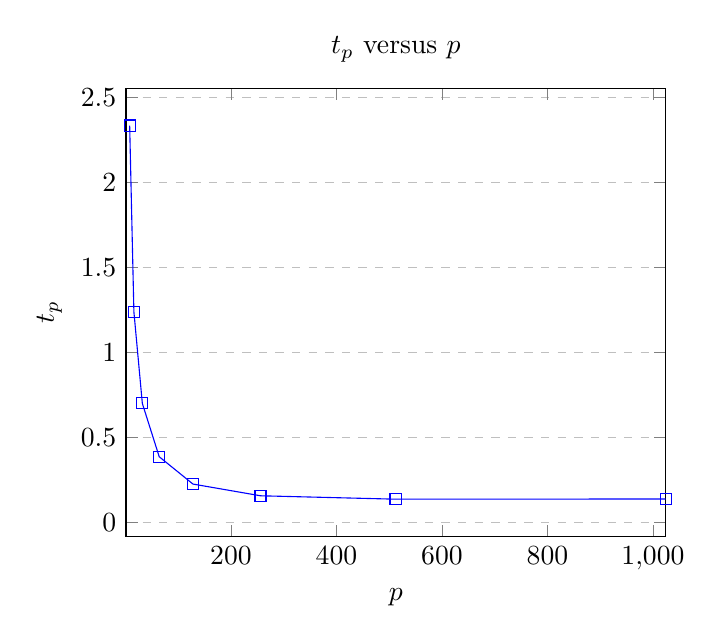
\begin{tikzpicture}
  \begin{axis}[title={$t_p$ versus $p$},xlabel={$p$},ylabel={$t_p$},xmin=1, xmax=1024,legend pos=north west, ymajorgrids=true,grid style=dashed]
  \addplot[color=blue,mark=square]coordinates{(8,2.336)(16,1.240)(32,.7)(64,.386)(128,.225)(256,.156)(512,.136)(1024,.137)};
  \end{axis}
\end{tikzpicture}

\end{document}
